\documentclass[tikz, border=12pt]{standalone}
\usepackage{amsmath}
\usetikzlibrary{positioning, arrows.meta}
\begin{document}
\begin{tikzpicture}[
    font=\sffamily,
    node distance=10mm and 8mm,
    card/.style={rectangle, rounded corners=6pt, draw=#1!55!black, thick,
        fill=#1!7, minimum width=5.6cm, minimum height=6.4cm,
        text width=5.0cm, align=center, inner sep=8pt},
]

\node[font=\sffamily\bfseries\LARGE, text=orange!45!black, anchor=north west]
    (title) at (0,0) {Derivative and Gradient Interpretation};

\node[below=6mm of title.west, anchor=north west, text width=17cm, align=left]
    (subtitle) {\textcolor{red!45!black}{\bfseries Optimization uses gradients to decide how a design should change to improve performance.}};

\node[card=blue, below=of subtitle.west, anchor=north west] (single)
    {\textcolor{black!70}{\bfseries Single-variable slope}\\[8pt]
     {\Large\itshape $\dfrac{df}{dx}$}\\[10pt]
     \textcolor{black!60}{\footnotesize rate of change of $f$ with respect to $x$}
     \par\vspace{8pt}
     \begin{tikzpicture}[baseline]
        \useasboundingbox (-0.3,-0.3) rectangle (3.4,2.6);
        \draw[-{Stealth[length=2mm]}] (-0.1,0) -- (3.2,0);
        \draw[-{Stealth[length=2mm]}] (0,-0.1) -- (0,2.4);
        \draw[thick, blue!60!black, domain=0:3, samples=40] plot (\x, {0.25*\x*\x});
        \draw[thick, red!70!black] (0.7,0.1) -- (2.3,1.7);
        \fill (1.5,0.5625) circle (1.3pt);
     \end{tikzpicture}
     \par\vspace{4pt}
     \textcolor{gray}{\footnotesize one variable}};

\node[card=orange, right=of single] (grad)
    {\textcolor{orange!55!black}{\bfseries Gradient}\\[8pt]
     {\Large\itshape $\nabla f(x)$}\\[10pt]
     \textcolor{orange!55!black}{\footnotesize collects partial derivatives for all design variables}
     \par\vspace{8pt}
     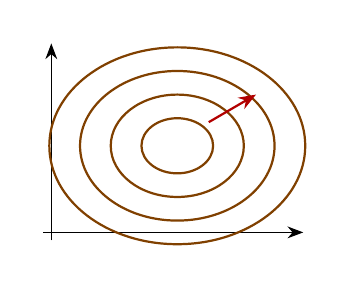
\begin{tikzpicture}[baseline]
        \useasboundingbox (-0.3,-0.3) rectangle (3.4,2.6);
        \draw[-{Stealth[length=2mm]}] (-0.1,0) -- (3.2,0);
        \draw[-{Stealth[length=2mm]}] (0,-0.1) -- (0,2.4);
        \foreach \r in {0.35,0.65,0.95,1.25}
          \draw[orange!50!black, thick] (1.6,1.1) ellipse ({\r*1.3} and {\r});
        \draw[-{Stealth[length=2.2mm]}, thick, red!70!black] (2.0,1.4) -- (2.6,1.75);
     \end{tikzpicture}
     \par\vspace{4pt}
     \textcolor{gray}{\footnotesize many variables}};

\node[card=green, right=of grad] (interp)
    {\textcolor{green!30!black}{\bfseries Interpretation}\\[10pt]
     \textcolor{green!30!black}{points in the direction of steepest increase}
     \par\vspace{20pt}
     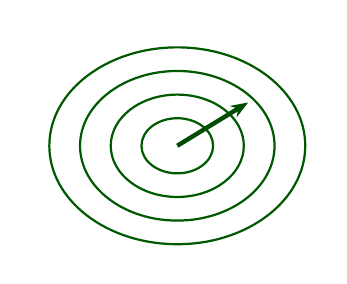
\begin{tikzpicture}[baseline]
        \useasboundingbox (-0.3,-0.3) rectangle (3.4,2.6);
        \foreach \r in {0.35,0.65,0.95,1.25}
          \draw[green!35!black, thick] (1.6,1.1) ellipse ({\r*1.3} and {\r});
        \draw[-{Stealth[length=2.2mm]}, ultra thick, green!30!black] (1.6,1.1) -- (2.5,1.65);
     \end{tikzpicture}};

\end{tikzpicture}
\end{document}
